% ==================================================================
\section{问题三：可解释性情感预测}\label{sec:q3}
% ==================================================================

问题三不再训练新的网络。解释层直接挂在第\ref{sec:base}章的预测网络外面，网络结构和参数都不改动，这样才能保证“解释的”就是“预测用的”那个模型。

\subsection{把“可解释”落实成可检验的输出}

题目对可解释性的要求是：说明本次判断主要依据了哪些输入，包括模态间的作用差异、主要参考模态，以及各模态中与判断密切相关的局部片段，并且证据能对应到原始材料。我们把它拆成四层，见表\ref{tab:layers}。

\begin{table}[htbp]
\centering
\caption{解释框架的四个层次}
\label{tab:layers}
\begin{tabular}{clll}
\toprule
层次 & 内容 & 主口径 & 输出 \\
\midrule
L0 & 回指 & 帧 $\leftrightarrow$ 词元，式(\ref{eq:align}) & 帧号对应的原文词 \\
L1 & 模态作用程度 & 干预式归因 & $s_l,s_a,s_v$，主导模态，裕度 $\mu$ \\
L2 & 片段级定位 & 滑动窗口遮蔽扫描 & 各模态逐帧重要性 $\mathrm{Imp}_m(t)$ \\
L3 & 证据呈现 & 回指 + 相对位置 & 文本词组；语音、视觉的词级锚点 \\
\bottomrule
\end{tabular}
\end{table}

这里有一个关键的取舍：结论一律由扰动实验给出，注意力权重只用来生成候选和做交叉检验。理由在第\ref{sec:noattn}节展开。

\subsection{L0：帧与词元的回指}

第\ref{sec:align}节已经证明50个序列位置是词级对齐的：第 $t$ 帧对应 $\texttt{input\_ids}$ 的第 $t$ 个词元。因此任何一帧都可以经 \texttt{tokenizer.decode} 还原成原文的词，不需要任何估计。

回指时有一条必须遵守的约束：证据只能从有效帧里选。文本限于实词区间 $[1,L)$，排除 \texttt{[CLS]}、\texttt{[SEP]} 和 \texttt{[PAD]}；语音、视觉限于帧号小于 $L_m$ 的帧。否则填充帧会被当成“关键证据”。这个坑我们实际踩过：第一版解释卡里出现过“\texttt{[PAD] [PAD] [PAD]}”这样的“证据”。原因前面也提到过，文本特征是上下文表示，补齐位置上的向量并不为零，遮蔽它们同样会让输出变化。

对语音和视觉，由于缺少逐词时间戳，我们给出“第 $t$ 个词元处”的词级锚点，同时给出相对位置 $t/L_m$，方便回到原始视频中按说话进度大致定位。

\subsection{L1：干预式模态归因}

对样本 $\mathbf{x}$，把模态 $m$ 按训练时的缺失注入方式整条遮蔽，记为 $\mathbf{x}_{\setminus m}$，比较遮蔽前后的输出：
\begin{align}
\Delta_m^{reg}&=\big|\hat y_{reg}(\mathbf{x})-\hat y_{reg}(\mathbf{x}_{\setminus m})\big|,\label{eq:dreg}\\
\Delta_m^{cls}&=\mathrm{KL}\Big(p(c\,|\,\mathbf{x})\ \big\|\ p(c\,|\,\mathbf{x}_{\setminus m})\Big),\label{eq:dcls}
\end{align}
前者衡量强度预测的偏移，后者衡量极性分布的变化。模态作用程度取分类口径归一化：
\begin{equation}\label{eq:share}
s_m=\frac{\Delta_m^{cls}}{\sum_{m'}\Delta_{m'}^{cls}},\qquad \sum_m s_m=1,\qquad
m^{*}=\arg\max_m s_m,\qquad \mu=s_{(1)}-s_{(2)},
\end{equation}
其中 $m^*$ 为主要参考模态，$s_{(1)}$、$s_{(2)}$ 为从大到小排列的前两个作用程度，$\mu$ 称为判定裕度。回归口径 $\Delta_m^{reg}$ 同时输出，作为辅助参考。

之所以额外报告裕度 $\mu$，是因为“主导模态是文本”这句话本身信息量有限：$s_l=0.95$ 和 $s_l=0.40$ 都会得出同一个结论，但含义差别很大。$\mu$ 小说明两个模态的作用接近，这时读者就不应把“主导模态”看得太重。

这里用遮蔽而不用梯度类方法（如积分梯度\cite{sundararajan2017ig}），还有一个本题特有的原因。积分梯度需要一个“基线输入”，而缺失场景下什么样的输入算“没有信息”本身就不好定义；遮蔽后的输入则正是模型训练时见过的缺失形态（假设(4)的说明），输出变化更可信。

\subsection{L2：片段重要性扫描}

用宽度为 $w$ 的窗口在模态 $m$ 的有效帧上滑动，只遮蔽窗口 $[t,t+w)$ 内的帧，记为 $\mathbf{x}^{[t,t+w)}_{\setminus m}$，定义第 $t$ 帧的片段重要性为
\begin{equation}\label{eq:imp}
\mathrm{Imp}_m(t)=\Big|\hat y_{reg}(\mathbf{x})-\hat y_{reg}\big(\mathbf{x}^{[t,t+w)}_{\setminus m}\big)\Big|
+\Big|p_{(1)}(\mathbf{x})-p_{(1)}\big(\mathbf{x}^{[t,t+w)}_{\setminus m}\big)\Big|,
\end{equation}
其中 $p_{(1)}$ 为遮蔽前预测类别的概率。第一项反映强度的变化，第二项反映对原判断的动摇程度。对主导模态取 $\mathrm{Imp}_m(t)$ 最大的若干帧作为关键证据帧，再经 L0 回指到原文词组或词级锚点。解释层的参数见表\ref{tab:xaiparam}。

\begin{table}[htbp]
\centering
\caption{解释层的主要参数}
\label{tab:xaiparam}
\begin{tabular}{>{\raggedright\arraybackslash}p{4.2cm}>{\raggedright\arraybackslash}p{8.6cm}}
\toprule
参数 & 设置 \\
\midrule
模态遮蔽方式 & 与训练时的缺失注入一致：语音、视觉置零，语言替换为 \texttt{[UNK]} 向量 \\
候选帧范围 & 文本 $[1,L)$；语音、视觉 $t<L_m$ \\
窗口宽度 $w$、证据帧数 $k$、稳定性检验噪声强度 & \todo{从配置文件抄录} \\
\bottomrule
\end{tabular}
\end{table}

\subsection{为什么不用注意力，以及融合层的等价重写}\label{sec:noattn}

式(\ref{eq:alpha})(\ref{eq:beta})中的 $\alpha$、$\beta$ 看上去就是现成的“解释”：它告诉我们语言的每个词关注了语音、视觉的哪些帧。但文献\cite{jain2019attention}的实验表明，注意力权重与预测的因果贡献并不必然一致，换一组差别很大的注意力分布，预测可以几乎不变。所以本文的结论全部来自扰动实验，注意力只做两件事：为片段扫描提供候选，以及与扰动结果做交叉检验。

即便只用来交叉检验，也得先把注意力取出来，这里遇到了一个工程问题。融合层使用的是 PyTorch 的 \texttt{TransformerDecoderLayer}，它内部调用注意力时设置了 \texttt{need\_weights=False}，即使挂上前向钩子，拿到的也只是 \texttt{None}。我们用显式的解码层重写了 \texttt{CrossModalFusion}，子模块命名与官方实现完全一致，因此可以直接加载原来训练好的参数。为了证明重写后的层与原层等价，做了三项检查，见表\ref{tab:equiv}。

\begin{table}[htbp]
\centering
\caption{重写融合层的等价性检查}
\label{tab:equiv}
\begin{tabular}{ll}
\toprule
检查项 & 结果 \\
\midrule
与原层的输出差异 & 最大绝对差 $4.77\times10^{-7}$（float32 舍入量级） \\
\texttt{state\_dict} 键名 & 完全不变，原检查点可直接加载 \\
开启注意力输出对预测的影响 & 逐元素相等，$\max|\Delta\hat y_{reg}|=0$ \\
\bottomrule
\end{tabular}
\end{table}

做这三项检查的原因很简单：可解释性分析报告的必须是真正在用的那个模型，而不是一个行为略有不同的近似副本，否则“解释”和“预测”就对不上了。

\subsection{解释质量的量化检验}

解释本身也需要被检验。我们用三个指标衡量解释的质量，结果见表\ref{tab:xaiquality}。
\begin{itemize}
\item \textbf{忠实性比值}：遮蔽重要性最高的 $k$ 个证据帧所引起的预测变化，除以遮蔽 $k$ 个随机有效帧所引起的预测变化。比值越大，说明挑出来的证据确实比随便挑的帧更重要。
\item \textbf{稳定性}：对输入加入微小噪声后重新计算重要性曲线，与原曲线的 Spearman 秩相关系数。越接近1，说明解释不会因为微小扰动而大幅改变。
\item \textbf{充分性偏移}：只保留重要性最高的3帧、遮蔽其余帧时，预测相对原预测的偏移量。越小说明少数证据帧就足以支撑原判断。
\end{itemize}

\begin{table}[htbp]
\centering
\caption{解释质量指标}
\label{tab:xaiquality}
\begin{tabularx}{\textwidth}{lcX}
\toprule
指标 & 数值 & 含义 \\
\midrule
忠实性比值 & 2.88 & 遮蔽 top-$k$ 证据造成的预测变化是随机帧的2.88倍 \\
稳定性（Spearman） & 0.9973 & 输入加噪后重要性曲线几乎不变 \\
充分性偏移 & 0.7068 & 只保留 top-3 帧时预测的偏移量 \\
\bottomrule
\end{tabularx}
\end{table}

前两项的结果比较理想：挑出的证据明显比随机帧重要，而且解释很稳定。第三项则提醒我们，只留3帧时预测偏移了0.7068，说明少数几帧并不足以单独支撑判断，模型依赖的信息是分散在整句中的。这与第\ref{sec:factor}节看到的语言高冗余是一致的。所以对文本证据更准确的读法是“模型最依赖的区域”，而不是“决定情感的那几个词”。

\subsection{三模态作用差异}

在验证集的192条样本上统计模态作用程度，结果见表\ref{tab:modshare}。

\begin{table}[htbp]
\centering
\caption{验证集（$n=192$）上的三模态作用程度}
\label{tab:modshare}
\begin{tabular}{lccc}
\toprule
 & 文本 & 语音 & 视觉 \\
\midrule
平均作用程度 $\bar s_m$ & \textbf{0.871} & 0.049 & 0.080 \\
作为主导模态的样本占比 & \textbf{92\%} & 4\% & 5\% \\
\bottomrule
\end{tabular}
\end{table}

注：占比经四舍五入，合计略超100\%。

这是我们最看重的一次交叉验证。干预式归因是在单个样本上做的，第\ref{sec:ablation}节的模态消融是在整个数据集上重新评测的，两条技术路线完全不同，却给出了同一个答案：语言是主导。这说明归因的口径是可信的。

表中还有一个值得注意的细节：视觉的平均作用程度（0.080）高于语音（0.049），可模态消融里去掉语音的损失（F1 $-3.1$）反而比去掉视觉（$+2.5$）大。两者并不矛盾。作用程度衡量的是“遮掉之后输出变了多少”，并不区分变得更准还是更差；视觉让输出变动较多，但这种变动未必朝着正确的方向，去掉视觉后 F1 略升也说明它带来的一部分是噪声。

\subsection{典型样本的解释}\label{sec:card}

图\ref{fig:interp}展示了测试集中的几条样本。左图是第0号样本三个模态的片段重要性曲线，横轴是帧号（即词元序号），竖线标出了各模态的关键证据帧；中图是第0～5号样本的模态作用程度；右图是这6条样本各模态的 $\Delta^{cls}$。

\begin{figure}[htbp]
\centering
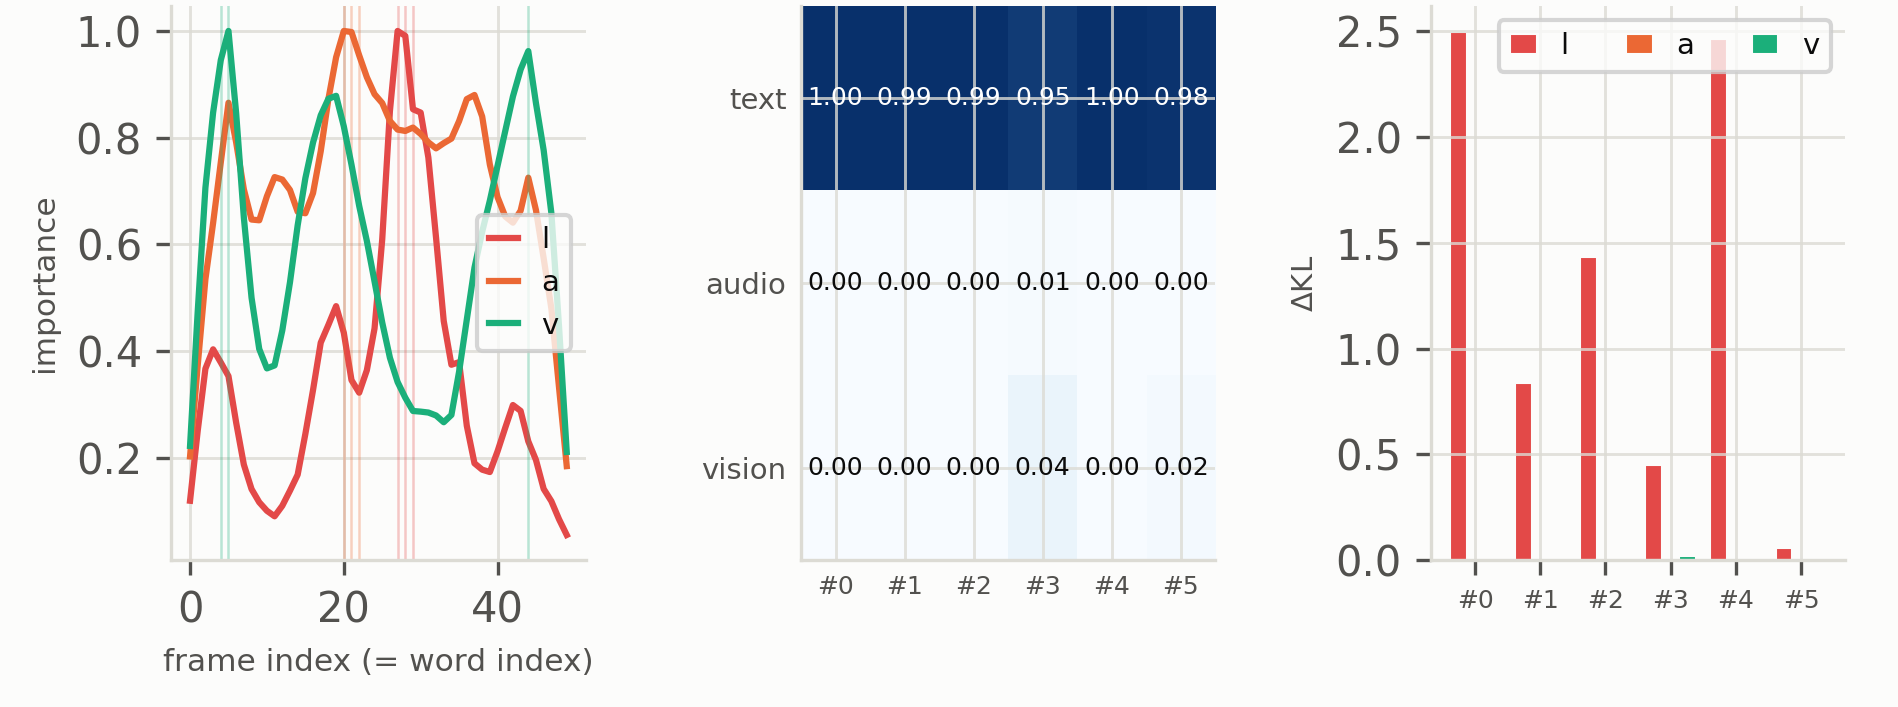
\includegraphics[width=\textwidth]{figures/fig_interpret.png}
\caption{测试样本的解释结果。左：第0号样本的片段重要性（l、a、v 分别为文本、语音、视觉）；中：第0～5号样本的模态作用程度 $s_m$；右：各模态遮蔽后的 $\Delta^{cls}$}
\label{fig:interp}
\end{figure}

从中图看，6条样本的文本作用程度都在0.95以上；语音、视觉只在第3号（视觉0.04、语音0.01）和第5号（视觉0.02）样本上有一点份额。右图说明文本主导的强弱在样本之间差别很大：第0号和第4号遮掉文本后 $\Delta^{cls}$ 接近2.5，第5号只有0.05左右，尽管后者的文本作用程度也有0.98。这正是需要同时看作用程度和绝对效应量的原因：作用程度是相对值，只说明“谁更重要”，而 $\Delta^{cls}$ 说明“整体有多重要”。

左图中文本的重要性在第27～29帧附近出现尖峰，这几帧就是该样本的文本关键证据，回指后即为对应位置的原文词组。

题目要求的解释卡包含预测结果、三模态作用程度、主要参考模态和关键证据定位。以附件4中可在附件2找回真值的第12号样本为例，解释卡如表\ref{tab:card}所示。

\begin{table}[htbp]
\centering
\caption{解释卡示例：附件4第12号样本}
\label{tab:card}
\begin{tabular}{>{\raggedright\arraybackslash}p{3.2cm}>{\raggedright\arraybackslash}p{9.6cm}}
\toprule
字段 & 内容 \\
\midrule
预测极性 & Negative（负向）；附件2中的真值同为 Negative \\
预测强度 & $-1.114$；真值 $-0.667$ \\
主要参考模态 & 文本；判定裕度 $\mu=$ \todo{见 json} \\
三模态作用程度 & $s_l=$ \todo{见 json}，$s_a=$ \todo{见 json}，$s_v=$ \todo{见 json} \\
文本关键证据 & “an individual previously”（词元位置 \todo{见 json}） \\
语音、视觉锚点 & 与文本证据同位置的帧，相对位置 $t/L_m=$ \todo{见 json} \\
复核方法 & 按帧号取 \texttt{input\_ids}，用 \texttt{tokenizer.decode} 还原原文；在原始视频中找到说出该词组的时刻，回看对应的语音与表情 \\
\bottomrule
\end{tabular}
\end{table}

\subsection{附件4的预测与解释结果}\label{sec:att4}

附件4的20条样本三模态完整，按与附件2相同的预处理送入网络，每条输出极性、强度、三模态作用程度、主导模态及裕度、关键证据帧和回指词组。结果分布见图\ref{fig:att4}，逐条结果见附录\ref{app:att4}，完整解释卡存于 attachment4\_explanations.json。

\begin{figure}[htbp]
\centering
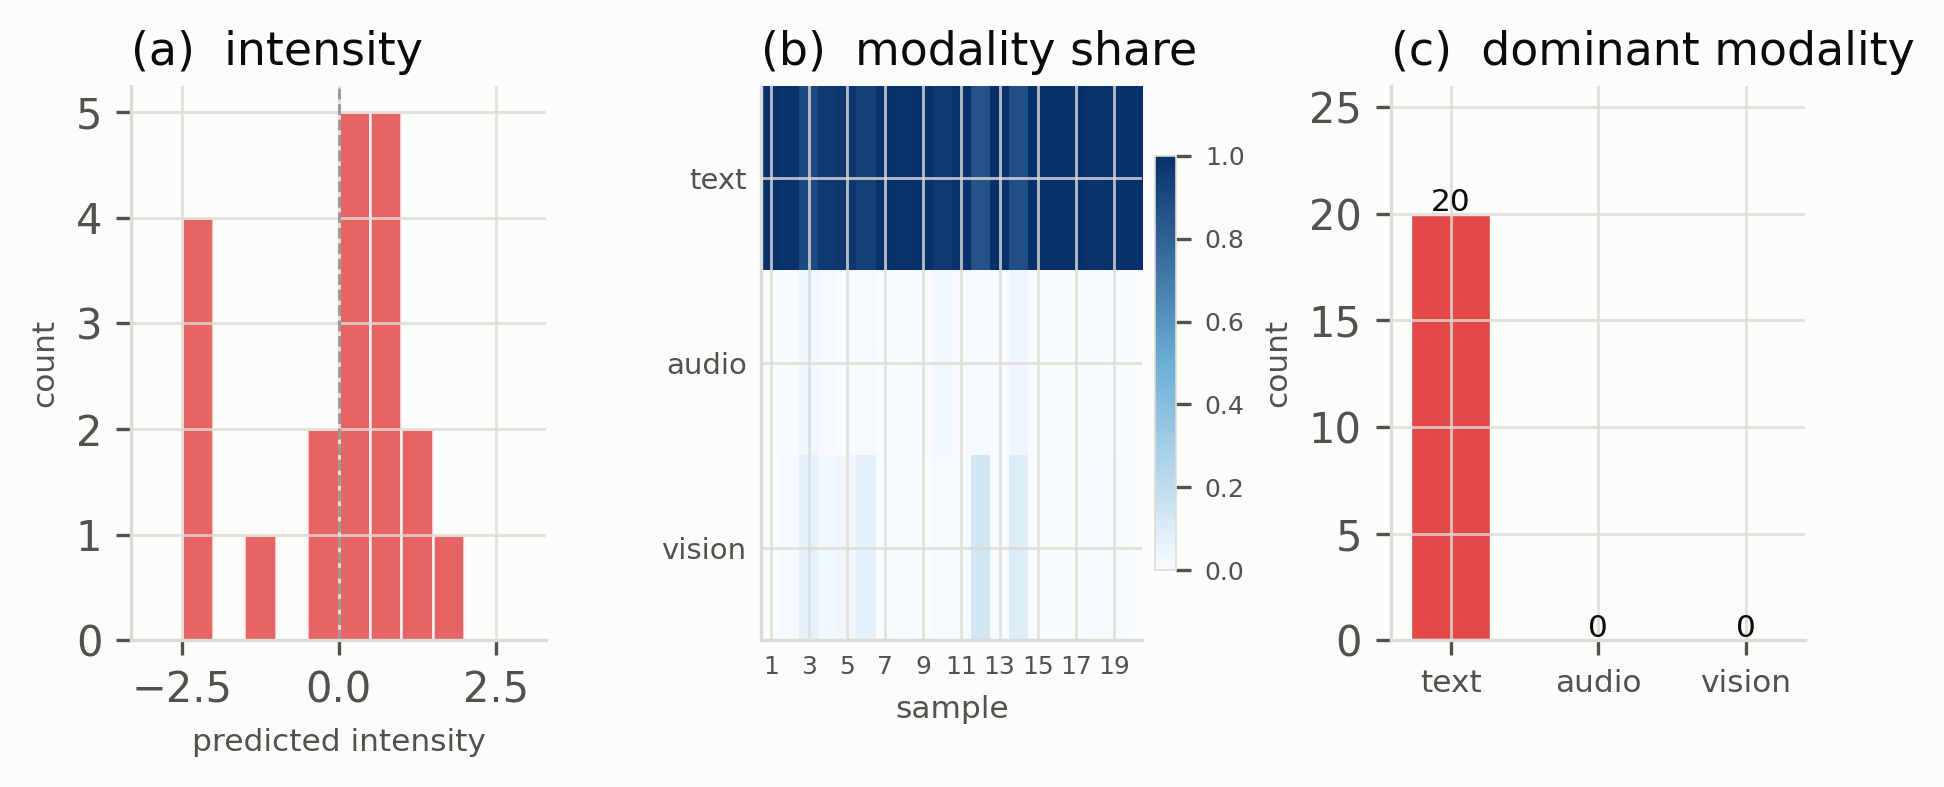
\includegraphics[width=\textwidth]{figures/fig_att4.png}
\caption{附件4推理结果：(a) 预测强度分布；(b) 各样本的模态作用程度；(c) 主导模态统计}
\label{fig:att4}
\end{figure}

20条样本的主导模态全部是文本，判定裕度均大于0.15，也就是说模型对每条样本都有明确的模态偏好。视觉在个别样本上占到了一定比例（图\ref{fig:att4}(b)中的浅色格），但都没有达到主导。预测强度的分布偏向两端，有4条落在$-2$以下的强负向区间。

附件4没有标签，但其中5条可以按编号在附件2里精确找回真值，可以当作一个很小的检验集，结果见表\ref{tab:att4match}。

\begin{table}[htbp]
\centering
\caption{附件4中可找回真值的5条样本}
\label{tab:att4match}
\begin{tabular}{cccccl}
\toprule
样本 & 预测极性 & 真值极性 & 预测强度 & 真值强度 & 文本关键证据 \\
\midrule
03 & Negative & Negative & $-0.402$ & $-0.333$ & “justwest don” \\
07 & Positive & Positive & $+0.946$ & $+0.667$ & “topics growing hobby” \\
08 & Positive & Positive & $+0.827$ & $+0.333$ & “to tonight ,” \\
12 & Negative & Negative & $-1.114$ & $-0.667$ & “an individual previously” \\
15 & Positive & Positive & $+1.379$ & $+1.000$ & “their , transform” \\
\bottomrule
\end{tabular}
\end{table}

5条样本的极性全部判对，强度 MAE 为0.3334。

\subsection{错误归因}\label{sec:q3err}

\textbf{（1）强度被系统性放大。}表\ref{tab:att4match}中5条样本的预测强度，绝对值全部大于真值，平均高出约0.33，强度 MAE 几乎全部来自这种同方向的偏差，例如08号预测$+0.827$，真值只有$+0.333$。样本只有5条，还不能下定论，但方向一致这一点值得重视。一种可能的解释是：真值是多名标注者的平均，标注者意见不一时平均值会被拉向0，而模型学到的是“这类说法通常有多强”。如果这个偏差在验证集上也成立，可以在验证集上拟合一个斜率小于1的线性校准来修正。

\textbf{（2）文本证据不一定是“情感词”。}表\ref{tab:att4match}的证据里有标点和虚词（“to tonight ,”、“their , transform”），也有不完整的词形（“justwest don”，BERT 按子词切分，回指出来的可能是半个词）。这和上文充分性偏移的结论一致：文本帧是上下文表示，遮掉一个窗口去掉的不只是这几个词本身，还有它们承载的上下文信息。因此文本证据应当理解为“模型最依赖的位置”，阅读时最好结合前后文。

\textbf{（3）语音、视觉的证据只能到词级。}数据中没有逐词时间戳，我们给出的是词级锚点和相对位置，不是绝对秒数。这是数据本身的限制，我们没有用“平均词长乘总时长”去凑一个秒数，因为那样得到的数字无法复核。

\textbf{（4）解释暴露了模型对文本的高度依赖。}92\%的样本以文本为主导，这是模型的真实行为，解释如实反映了它。反过来说，如果某条样本的转写文本有错，模型很可能跟着出错，而这类样本的解释卡会显示“文本主导”，读者据此就能意识到应当先核对转写。这也是可解释性在实际使用中的价值所在。

\subsection{小结}

问题三在不改动网络的前提下，用“干预 + 回指”的方式给出了可量化、可复核的解释：模态作用程度由遮蔽后的输出变化归一化得到，关键证据由滑动窗口扫描定位，再借助帧—词元对应还原到原文。忠实性比值2.88、稳定性0.9973说明解释是可靠的；单样本归因与整体消融两条独立路线得到同一个结论，互相印证了口径的可信度。主要的不足在于语音、视觉只能定位到词级，以及模型存在放大情感强度的倾向。
